\documentclass[conference]{IEEEtran}
\IEEEoverridecommandlockouts
\usepackage{cite}
\usepackage{amsmath,amssymb,amsfonts}
% newtx is used by the repository build (Tectonic); fall back to Times where it is not installed.
\IfFileExists{newtxtext.sty}{\usepackage{newtxtext,newtxmath}}{\usepackage{mathptmx}}
\usepackage{graphicx}
\usepackage{booktabs}
\usepackage{tabularx}
\usepackage{array}
\usepackage{listings}
\usepackage{xcolor}
\usepackage[hidelinks]{hyperref}
\usepackage{url}
\usepackage{flafter}
\usepackage{float}
\usepackage{needspace}
\usepackage{balance}
\setcounter{dbltopnumber}{5}
\setcounter{totalnumber}{6}
\renewcommand{\dbltopfraction}{0.95}
\renewcommand{\dblfloatpagefraction}{0.85}
\setlength{\textfloatsep}{8pt plus 2pt minus 2pt}
\lstset{basicstyle=\ttfamily\scriptsize,breaklines=true,columns=fullflexible,keepspaces=true,frame=single,framerule=0.2pt,xleftmargin=2pt,xrightmargin=2pt,aboveskip=4pt,belowskip=4pt}
\clubpenalties 3 10000 10000 0
\newcolumntype{L}[1]{>{\raggedright\arraybackslash}p{#1}}
\hypersetup{pdftitle={SPIRA: Preparing Smart Homes from Online Orders via Retrieval-Augmented Inference over Synthetic Purchase-Intent Knowledge},pdfauthor={Jeewon Lee, Uijin Lee, Seojin Lee, Yejoon Kim}}
\title{SPIRA: Preparing Smart Homes from Online Orders via Retrieval-Augmented Inference over Synthetic Purchase-Intent Knowledge}
\author{
\IEEEauthorblockN{Jeewon Lee}
\IEEEauthorblockA{\small\textit{Dept. of Information Systems}\\\textit{Hanyang University}\\Seoul, Republic of Korea\\leejeewon916@gmail.com}
\and
\IEEEauthorblockN{Uijin Lee}
\IEEEauthorblockA{\small\textit{Dept. of Information Systems}\\\textit{Dept. of Food \& Nutrition}\\\textit{Hanyang University}\\Seoul, Republic of Korea\\smilelejn@gmail.com}
\and
\IEEEauthorblockN{Seojin Lee}
\IEEEauthorblockA{\small\textit{Dept. of Information Systems}\\\textit{Hanyang University}\\Seoul, Republic of Korea\\leeseojini0303@gmail.com}
\and
\IEEEauthorblockN{Yejoon Kim}
\IEEEauthorblockA{\small\textit{Dept. of Information Systems}\\\textit{Hanyang University}\\Seoul, Republic of Korea\\yejoonkim1340@gmail.com}
}
\IEEEaftertitletext{\vspace{-\baselineskip}{\centering\footnotesize CSE 406 Software Engineering --- Team SPIRA --- Submissions C and D (draft of 2026-11-23)\par}\vspace{0.5em}}
\begin{document}
\maketitle
\raggedbottom
\begin{abstract}
Online delivery brings products to the door, but users must still prepare the home for the situation those products indicate. \textbf{SPIRA} connects a shared order to household preparation through retrieval-augmented purchase-intent inference. Before launch there are no real purchase-intent records, so language-model agents from three companies generate synthetic order cases over 30 intents; two models from different companies label each case blindly, and batches pass a quality gate before they are embedded and loaded. For each shared order, the Server reads the screenshot, retrieves similar cases, and makes one intent judgment with a language model. Code then finds the time, limits tasks to the household's delegated devices, and publishes a versioned plan that the Home Hub pulls, executes, reads back, and restores. The home acts at only two moments: the time of the intended occasion and the moment a package is brought in. The user receives one card per preparation and can stop it or switch off a single line. Stops, switched-off lines, and person-made changes become household memory. This paper updates the requirements and specifications of Submission B to the current design and adds the architecture, implementation, and use cases.
\end{abstract}
\begin{IEEEkeywords}smart home, purchase intent, synthetic knowledge, retrieval-augmented generation, household preparation\end{IEEEkeywords}

\section{Introduction}
\subsection{Motivation}
A delivery service brings products to the door. Household preparation still requires the user's effort. After an order arrives, the user must decide how each item should be stored, treated, or used. The same strawberry should be handled differently when it is an ordinary grocery item and when it is intended for decorating cupcakes at a birthday party. These decisions are small individually, but they accumulate at the exact time when online shopping is supposed to reduce effort.

A second burden appears when several purchased items indicate a future occasion. Party decorations, children's tableware, cupcake ingredients, and drinks together suggest a household situation. Users must translate that situation into separate actions such as cleaning before guests arrive, preparing child-safety settings, changing lighting and media, and placing an oven in a ready state. Existing smart-home routines automate these actions only after the user has recognized the situation and configured the rules. SPIRA connects purchase-intent evidence to situation-driven home preparation, with bounded item-handling guidance as a supporting responsibility.

\subsection{Problem Statement}
Current services stop at separate boundaries. Commerce systems know what was ordered but do not observe how the order is used inside the home. Delivery tracking stops at the door. Appliance applications know device state, but not why a set of incoming products matters. Rule-based platforms execute a trigger-action pair only after the user has authored it.

The missing responsibility is a bounded decision process that connects an order to a household situation and appropriate preparation. Before deployment, real household purchase-intent records do not exist. Synthetic purchase-intent knowledge supplies retrievable cases for this cold-start problem, while its utility and bias require evaluation. Three risks must be controlled: over-interpreting ordinary orders, proposing impossible or unsafe commands, and turning convenience into intrusive automation.

\subsection{Proposed Solution}
SPIRA treats one shared order as one episode and processes it in seven Server stages, S1--S7:

\begin{lstlisting}
S1 read screenshots -> items (label, mask sensitive)
S2 context + retrieve similar synthetic cases (RAG)
S3 one intent judgment (30 intents, none, unclassified)
S4 time by code (find_time) + need-first tasks
S5 safety checks, merge, versioned plan, cards
S6 App and Hub APIs (the Hub pulls the plan)
-- Home Hub: trigger, execute, read back, restore --
S7 per-card verdict and per-line feedback -> memory
\end{lstlisting}
The language model is called only in S1 (reading), S3 (intent), and S4 (tasks), plus a separate tagging call when a calendar arrives. Code owns retrieval, time, validation, plan state, and execution. A question, confirmation request, refusal, or empty answer from the model is treated as a format error: the stage retries once and then uses its default, such as ``no intent.'' The service therefore never asks the user back. Most orders end with no intent and zero tasks, which is a normal result.

\textbf{Scope rule.} The home moves at two moments only: (1) at the time of the intent, for situation preparation such as cleaning, child-safety mode, mood screen, light, and music, or an oven standby; and (2) when a package is brought in, for per-item tasks that are harmless whenever the item is used, such as a fridge care notice. Trigger kinds are limited to \texttt{time}, \texttt{package.brought\_in}, \texttt{guest\_arrived}, and \texttt{event\_end}.

\subsection{Representative Scenario and Prototype Scope}
The first end-to-end scenario is a child's birthday party. On Thursday evening the user shares an order with pink and purple balloons, a princess cake topper, party hats, cupcake mix, icing pens, strawberries, cream, juice, disposable tableware, detergent, and lotion. The calendar says only ``Saturday 14:00 birthday.'' The order suggests a princess theme, visiting children, and a cupcake activity; detergent and lotion stay outside the bundle. SPIRA shows one card, displays strawberry guidance on the fridge screen when the package is brought in, cleans and enables a child-safety mode 30 minutes before guests, sets mood light and screen when the first guest arrives, prepares an oven standby (a person starts cooking), and restores only what it changed when the party ends.

The prototype uses an Android phone for the App, a Mac process for the Home Hub, and a test home that simulates appliances over MQTT. A physical Tapo light is planned. Every surface distinguishes physical integration from simulation.

\subsection{Related Software and Research}
Shopping-mission research shows that baskets can represent a purpose rather than a set of categories \cite{ref1}. Bundle-recommendation work separates intent-related products from unrelated products in a session \cite{ref2}, and adaptive in-context learning uses similar sessions as examples for bundle generation \cite{ref3}. COSMO generates purchase-intent knowledge with large language models at commerce scale and verifies part of it with human annotation \cite{ref4}. SAGE shows that purely synthetic data can replace private data as the retrieval corpus of retrieval-augmented generation \cite{ref5}; SPIRA uses synthetic cases for a different reason, because real household records do not yet exist. Because language-model evaluators favor their own generations \cite{ref16}, SPIRA labels each case blindly with two models from different companies. LaMP retrieves user records for personalization \cite{ref6}. Sasha studies goal-oriented smart-home planning \cite{ref7}, and HomeBench documents failures on invalid device instructions that motivate deterministic capability and safety validation \cite{ref8}.

\section{Requirements}
The requirements of Submissions A and B remain the basis. This section restates them where the design changed after Submission B. The Server stage that satisfies each group is shown in brackets.

\subsection{Household Setup and Order Intake}
\textbf{Household Capability Registration [S6, Hub].} The system shall let a household register its devices, rooms, display names, and the commands it delegates to SPIRA. Actions marked \texttt{never} shall be shown as not delegated and shall not be selectable. The user shall be able to pause and resume SPIRA at any time.

\textbf{User-Controlled Order Sharing [S1].} The system shall accept screenshots of an order screen, a cart, or a product page through the Android share sheet. Captures within 8 hours form one order, and the order is read once after 10 quiet minutes. Unchecked, sold-out, and recommended items shall be skipped. Duplicate items and repeated captures shall not create duplicate episodes.

\textbf{Structured Order Extraction [S1].} For each order, the system shall extract item names, a short item type, quantity, product group, and attributes copied from the product name or options. The item type shall keep an occasion or use word (e.g., ``birthday balloon'') and drop brand, flavour, colour, and character. A theme attribute shall be recorded only for decorating goods. Items in five sensitive categories shall be masked, and images shall be deleted after extraction.

\subsection{Context and Intent}
\textbf{Bounded Context Assembly [S2].} The system shall assemble the order time, the household's types, unusual items relative to its last 90 days, calendar tags, and retrieved synthetic cases. Calendar titles shall never be stored; only tags and a change fingerprint are kept. Device lists and household memory shall not enter intent judgment.

\textbf{Retrieval of Synthetic Cases [S2].} The system shall embed the item types with BGE-M3 \cite{ref15} and retrieve cases above a similarity floor of 0.70, with small bonuses for a matching calendar tag (+0.05) and household type (+0.03). It shall pass at most 50 neighbours and three representative cases, and pass no knowledge-base block when fewer than five neighbours remain. Intent counts shall be shown together with the knowledge base's base rate.

\textbf{One-Shot Intent Judgment [S3].} The system shall make one judgment that returns at most two bundles, each with one of 30 intents, \texttt{none}, or \texttt{unclassified}, a situation (event, theme, guests, activity), and the excluded items. Unknown details shall stay empty. A calendar event shall be linked only when its tags match the intent's related tags. Retrieval similarity and model confidence shall not authorize execution.

\subsection{Tasks and Plan}
\textbf{Need-First Task Generation [S4].} For each bundle, the system shall describe the household need first and map it to the household's delegated commands. Each task shall have a way: \texttt{run}, \texttt{standby} (a person starts the appliance), or \texttt{notice}. A bundle shall produce at most four lines. Zero tasks is valid.

\textbf{Time by Code [S4].} The language model shall never produce a time. Code shall look for the intent's time in the calendar, then a holiday calendar, then this household's habit; otherwise the tasks shall be held for up to 14 days.

\textbf{Per-Item Tasks [S4].} Per-item tasks shall come from a fixed table (fridge care notice, styler or shoe-care standby, super-freeze, mattress deodorising), shall be triggered by \texttt{package.brought\_in}, and shall be made only when exactly one matching device exists. Fridge notices shall be shown only for mistakes people commonly make, at most three per screen, and the same notice at most twice.

\textbf{Deterministic Plan Validation [S5].} Every action shall pass a server-side allow list per way. Commands containing deny words (start, ignite, heat, unlock, open, buy, order, pay, delete, reset) shall be dropped even if listed. Value ranges, rooms per action, and quiet hours for noisy devices shall be checked. Safety actions such as child lock or plug off shall be marked \texttt{protective}.

\textbf{Plan Versioning [S5].} Calendar changes, line changes, and stops shall publish a new plan version. Started work keeps its identifier and result; a stopped card is never revived.

\subsection{Execution and Recovery}
\textbf{Event-Driven, State-Aware Execution [Hub].} The Hub shall pull the current plan, wait for its triggers, recheck delegation and device state immediately before dispatch, and execute only delegated commands of the current version.

\textbf{Verification, Ownership, and Restoration [Hub].} After a command, the Hub shall read back the state and distinguish acceptance from observed effect. Ownership is tracked per changed property; any later change not made by SPIRA releases it, and released properties are never overwritten. A protective task is released only after an observed \texttt{event\_end}; a time fallback ends it without release and reports the item as withheld.

\subsection{Observation and Household Memory}
\textbf{Signal-Based Observation [S7].} Each card has one observation window. Confirmation signals come from the plan: a person starting an appliance left in standby, or an event trigger such as \texttt{guest\_arrived} actually occurring. Running as planned is not evidence. The verdict shall be \texttt{stopped}, \texttt{match}, or \texttt{unconfirmed}; silence shall never count as a match. Comparison with a household usage baseline is removed from the prototype.

\textbf{Household Memory [S7].} Each closed card with situation lines shall write one memory row: the items, intent, situation, what the home did, the verdict, and per-line feedback (\texttt{off}, \texttt{changed}, \texttt{kept}). S4 uses this memory; S3 does not. Lines switched off are left out of the same intent for 180 days. A household shall be able to list and delete each row.

\subsection{Interaction, Privacy, and Evaluation}
\textbf{Quiet and Explainable Interaction [S5, App].} One preparation shall be shown as one card, at most two per order and four lines per card, with no approval button. The App shall expose exactly three interventions: Stop on each card (end this preparation now, without asking for a reason), line off before the line starts, and household pause. There is no house-wide stop. A rationale view shall be assembled from stored values without calling the model again. Shared screens shall never name the occasion, guests, or theme.

\textbf{Privacy and Data Minimization.} Masked items store only group and quantity and never reach embedding, intent, tasks, notices, or rationale. Temporary images are deleted within one day, and device-state events after 14 days. Synthetic-case generation and labeling never receive real orders or household records.

\textbf{Evaluability.} The retrieval contribution shall be evaluated on new orders that are not in the knowledge base, under three conditions: no knowledge base (C0), knowledge base (C1), and knowledge base with household context (C2), each with a free Gemini model and Claude Sonnet 5.5, with the knowledge base fixed at version \texttt{kb-v1}. Synthetic results shall not be presented as evidence of real adoption.

\textbf{Demonstration Boundary.} The demonstration shall prioritize the birthday episode and an ordinary grocery order. Simulated and physical devices shall be labeled on every interface.

\section{Development Environment}
\subsection{Choice of Software Development Platform}
Development uses a MacBook Air (\texttt{Mac16,12}) with an Apple M4 processor, 10 CPU cores, 16 GB of memory, and macOS 26.5. The Server, database, Home Hub, and test home run on this machine with Docker for the Server and PostgreSQL. The Home Hub runs as a Mac process; the Galaxy S10 placement of Submission B was dropped on 2026-11-19 to simplify the demonstration. The App targets Android, because receiving shared screenshots requires the platform share intent, which is implemented in Kotlin.

Python 3.12 is used for the Server, Home Hub, and test home because these parts share HTTP handling, validation, and test utilities, and because the knowledge-base embedding package is a Python library. The App uses Flutter with Dart 3.14 so that sharing, cards, rationale, and settings live in one codebase. PostgreSQL 16 with pgvector stores episodes, plans, memory, and the synthetic-case index.

\textbf{Cost.} The prototype reuses the MacBook Air and existing Android phones, so its hardware cost is KRW 0; a Tapo light is the only planned new device. Synthetic cases are generated with team members' existing language-model subscriptions, so the knowledge base adds no cost. Runtime model calls are logged per call for later cost reporting. Deployment on Amazon Web Services is planned: one RDS for PostgreSQL instance with pgvector holding the server tables and a knowledge-base snapshot, an S3 bucket for screenshots with a one-day lifecycle, and a Server host with at least 4 GB of memory for BGE-M3. The database was estimated at USD 20--25 per month for a \texttt{db.t4g.micro} class; it is not deployed yet.

\subsection{Software in Use}
The Server uses FastAPI, Uvicorn, Pydantic, SQLAlchemy 2, Alembic, psycopg 3, pgvector, APScheduler, and the Anthropic SDK; the Hub and test home use FastAPI, httpx, SQLite, and Paho MQTT with a Mosquitto broker. Exact versions are pinned in each folder's project file. The knowledge base is built in a separate repository whose GitHub Actions workflow assembles, compares, gates, deduplicates, embeds with BGE-M3 \cite{ref15}, and loads cases. During development the knowledge base is served from a Neon PostgreSQL database through a read-only role. Official policies for Python, PostgreSQL, pgvector, and Flutter are cited in \cite{ref9}--\cite{ref14}.

\subsection{Task Distribution}
\begin{table}[H]
\caption{Task Distribution}
\centering
\footnotesize
\setlength{\tabcolsep}{2.5pt}
\renewcommand{\arraystretch}{1.08}
\begin{tabularx}{\columnwidth}{@{}L{0.17\columnwidth}L{0.16\columnwidth}X@{}}
\toprule
\textbf{Course role} & \textbf{Member} & \textbf{Work in the project} \\
\midrule
User & Uijin Lee & Synthetic purchase-intent knowledge base: case generation, blind labels, quality gate, loading, embedding package, shared lists \\
Customer & Seojin Lee & SPIRA Server (S1--S7), team contracts, retrieval tuning and evaluation \\
Software developer & Yejoon Kim & App (Flutter), Home Hub, test home (simulator) \\
Development manager & Jeewon Lee & Paper integration, README, architecture figure, deployment, knowledge-base automation node \\
\bottomrule
\end{tabularx}
\label{tab:tasks}
\end{table}

\section{Specifications}
One episode proceeds through intake and intent (S1--S3), tasks and plan (S4--S5), local execution (Hub), and observation and memory (S7).

\subsection{Order Intake and Intent Interpretation}
The App sends each shared screenshot with a stable source identifier; a repeated identifier returns the existing episode. Captures within 8 hours join one episode, and a quiet timer starts S1 ten minutes after the last capture. S1 calls the model once per quiet period with a strict JSON schema. Code then labels each item as \texttt{care} (may create a per-item task) or \texttt{clue} (used only inside an intent) from a product-group table, masks sensitive items, and merges duplicates.

S2 embeds the unmasked item types with the same function the knowledge base used (\texttt{embed\_basket}) and searches cases whose version is at most \texttt{KB\_VERSION}. Neighbours are scored by similarity plus context bonuses, and the block given to S3 lists intent counts beside the knowledge base's base share, so S3 can prefer intents that appear more often than usual.

\begin{figure}[!t]
\noindent\begin{minipage}{\columnwidth}
\begin{lstlisting}
judge(episode):
    items = unmasked(episode.items)
    if not items: return no_intent("all_masked")
    ctx = this_home(episode)        # types, unusual, tags
    kb  = search(embed_basket(types(items)),
                 floor=0.70, k=200, keep=50)
    if len(kb) < 5: kb = None
    out = llm_once("s3", items, ctx, kb, schema=S3)
    if not format_ok(out): out = llm_retry_once(...)
    if not format_ok(out): return no_intent("format")
    return out.bundles[:2]          # intent, situation
\end{lstlisting}
\end{minipage}
\end{figure}
S3's format check verifies the schema, intent identifiers, item references, and that situation values repeat the intent sentence. A calendar link is removed when its tags do not overlap the intent's related tags.

\subsection{Tasks and Plan Formation}
For each bundle, S4 first checks this household's memory: a stopped card for the same intent and tag set removes situation tasks, and lines switched off within 180 days are excluded. The time is found by code; the model receives the household's delegated device list and writes needs, then tasks.

\noindent\begin{minipage}{\columnwidth}
\begin{lstlisting}
find_time(bundle):
    for source in (calendar, holiday_calendar, habit):
        t = source.match(bundle)
        if t: return t
    return HOLD(days=14)   # card says time not found

plan(episode):
    for task in s4_tasks(episode) + item_tasks(episode):
        drop if cmd not in allow_list[task.way]
        drop if any(deny_word in cmd)
        drop actions in another room
        drop noisy time triggers in quiet hours
    merge(tasks); cards = one_per_bundle(max=2)
    publish_plan_version(tasks)  # Hub pulls it
\end{lstlisting}
\end{minipage}
Fridge notices are filtered by count and kept to three per screen. Card text comes from templates with verified slots instead of free model text. A version made only of cancellations stays in the pull until acknowledged.

\subsection{Local Execution and Recovery}
The Hub pulls \texttt{GET /v1/hub/plans} every 15 seconds and acknowledges each version; the Server never calls the Hub or the App. Triggers are evaluated locally from the test home's events and the clock. Immediately before dispatch the Hub rechecks that the plan version is current, the command is still delegated, and the device is available.

\begin{figure}[!t]
\noindent\begin{minipage}{\columnwidth}
\begin{lstlisting}
on_trigger(task):
    if not current(task) or not delegated(task.cmd):
        return report(task, "not_started")
    prior = read_state(task.devices)
    send(task.actions)
    effect = read_back(task.devices)
    own(task, changed_properties(prior, effect))
    report(task, effect)

on_end(task, observed_event_end):
    if task.protective and not observed_event_end:
        return report(task, "withheld_end_not_observed")
    restore(still_owned_properties(task))
\end{lstlisting}
\end{minipage}
\end{figure}
A card Stop reaches the Hub only as a newer plan version: unstarted work is cancelled, effects SPIRA still owns are restored, and person changes and person-started jobs are preserved.

\subsection{Observation, Memory, and Interaction}
S7 creates an observation window with each card. The window opens at the first confirmed start or at the scheduled start and closes on a stop, an observed \texttt{event\_end}, or the end time plus a fallback. Events are linked by device and time.

\noindent\begin{minipage}{\columnwidth}
\begin{lstlisting}
close_window(card):
    if card.stopped: verdict = "stopped"
    elif any_signal(card):   # standby started by a
        verdict = "match"     # person, or event seen
    else: verdict = "unconfirmed"
    feedback = {line: off | changed | kept}
    if card.has_situation_lines and intent != unclassified:
        write_memory_row(card, verdict, feedback)
\end{lstlisting}
\end{minipage}
The App polls cards every 30 seconds and shows at most one local notification per card update flagged \texttt{notify}. The rationale view reads stored evidence, intents, knowledge-base counts, tasks with devices and rooms, executions, and observations.

\subsection{Evaluation and Demonstration}
The evaluation varies only the input to S3 (C0, C1, C2) and the model, records intent or no-intent, bundle items, unsupported details, and output validity, and uses orders that are not in the knowledge base. Switches \texttt{KB\_MODE}, \texttt{HOME\_CONTEXT}, and \texttt{KB\_SAMPLE} select the conditions, and every model call is logged. Results are pending. The demonstration combines the birthday order and an ordinary grocery order, with labeled simulated and physical devices.

\section{Architecture Design and Implementation}
\subsection{Overall Architecture}
Fig.~\ref{fig:arch} shows the components and the data that flows between them. On the phone, the user shares order screenshots from a shopping app to the SPIRA App (Flutter), which sends them to the Server and receives preparation cards. The Server is a FastAPI application in Docker on Amazon EC2 inside a VPC; it contains S1--S7, sends items and context to the Claude API and receives intents and tasks in S1, S3, and S4, and stores episodes, memory, and the knowledge-base snapshot in Amazon RDS for PostgreSQL with pgvector. The Home Hub (Python) receives plans and returns events and results; it sends commands to home appliances and IoT devices over MQTT and receives their state. The knowledge base is built offline: Gemini, ChatGPT (Codex), and Claude agents generate cases and cross-labels, and GitHub Actions embeds them with BGE-M3 and loads cases and embeddings into the database. Arrows show the direction of data; the App and the Hub fetch cards and plans from the Server, which never calls them. The AWS deployment is planned.

\begin{figure*}[!t]
\centering
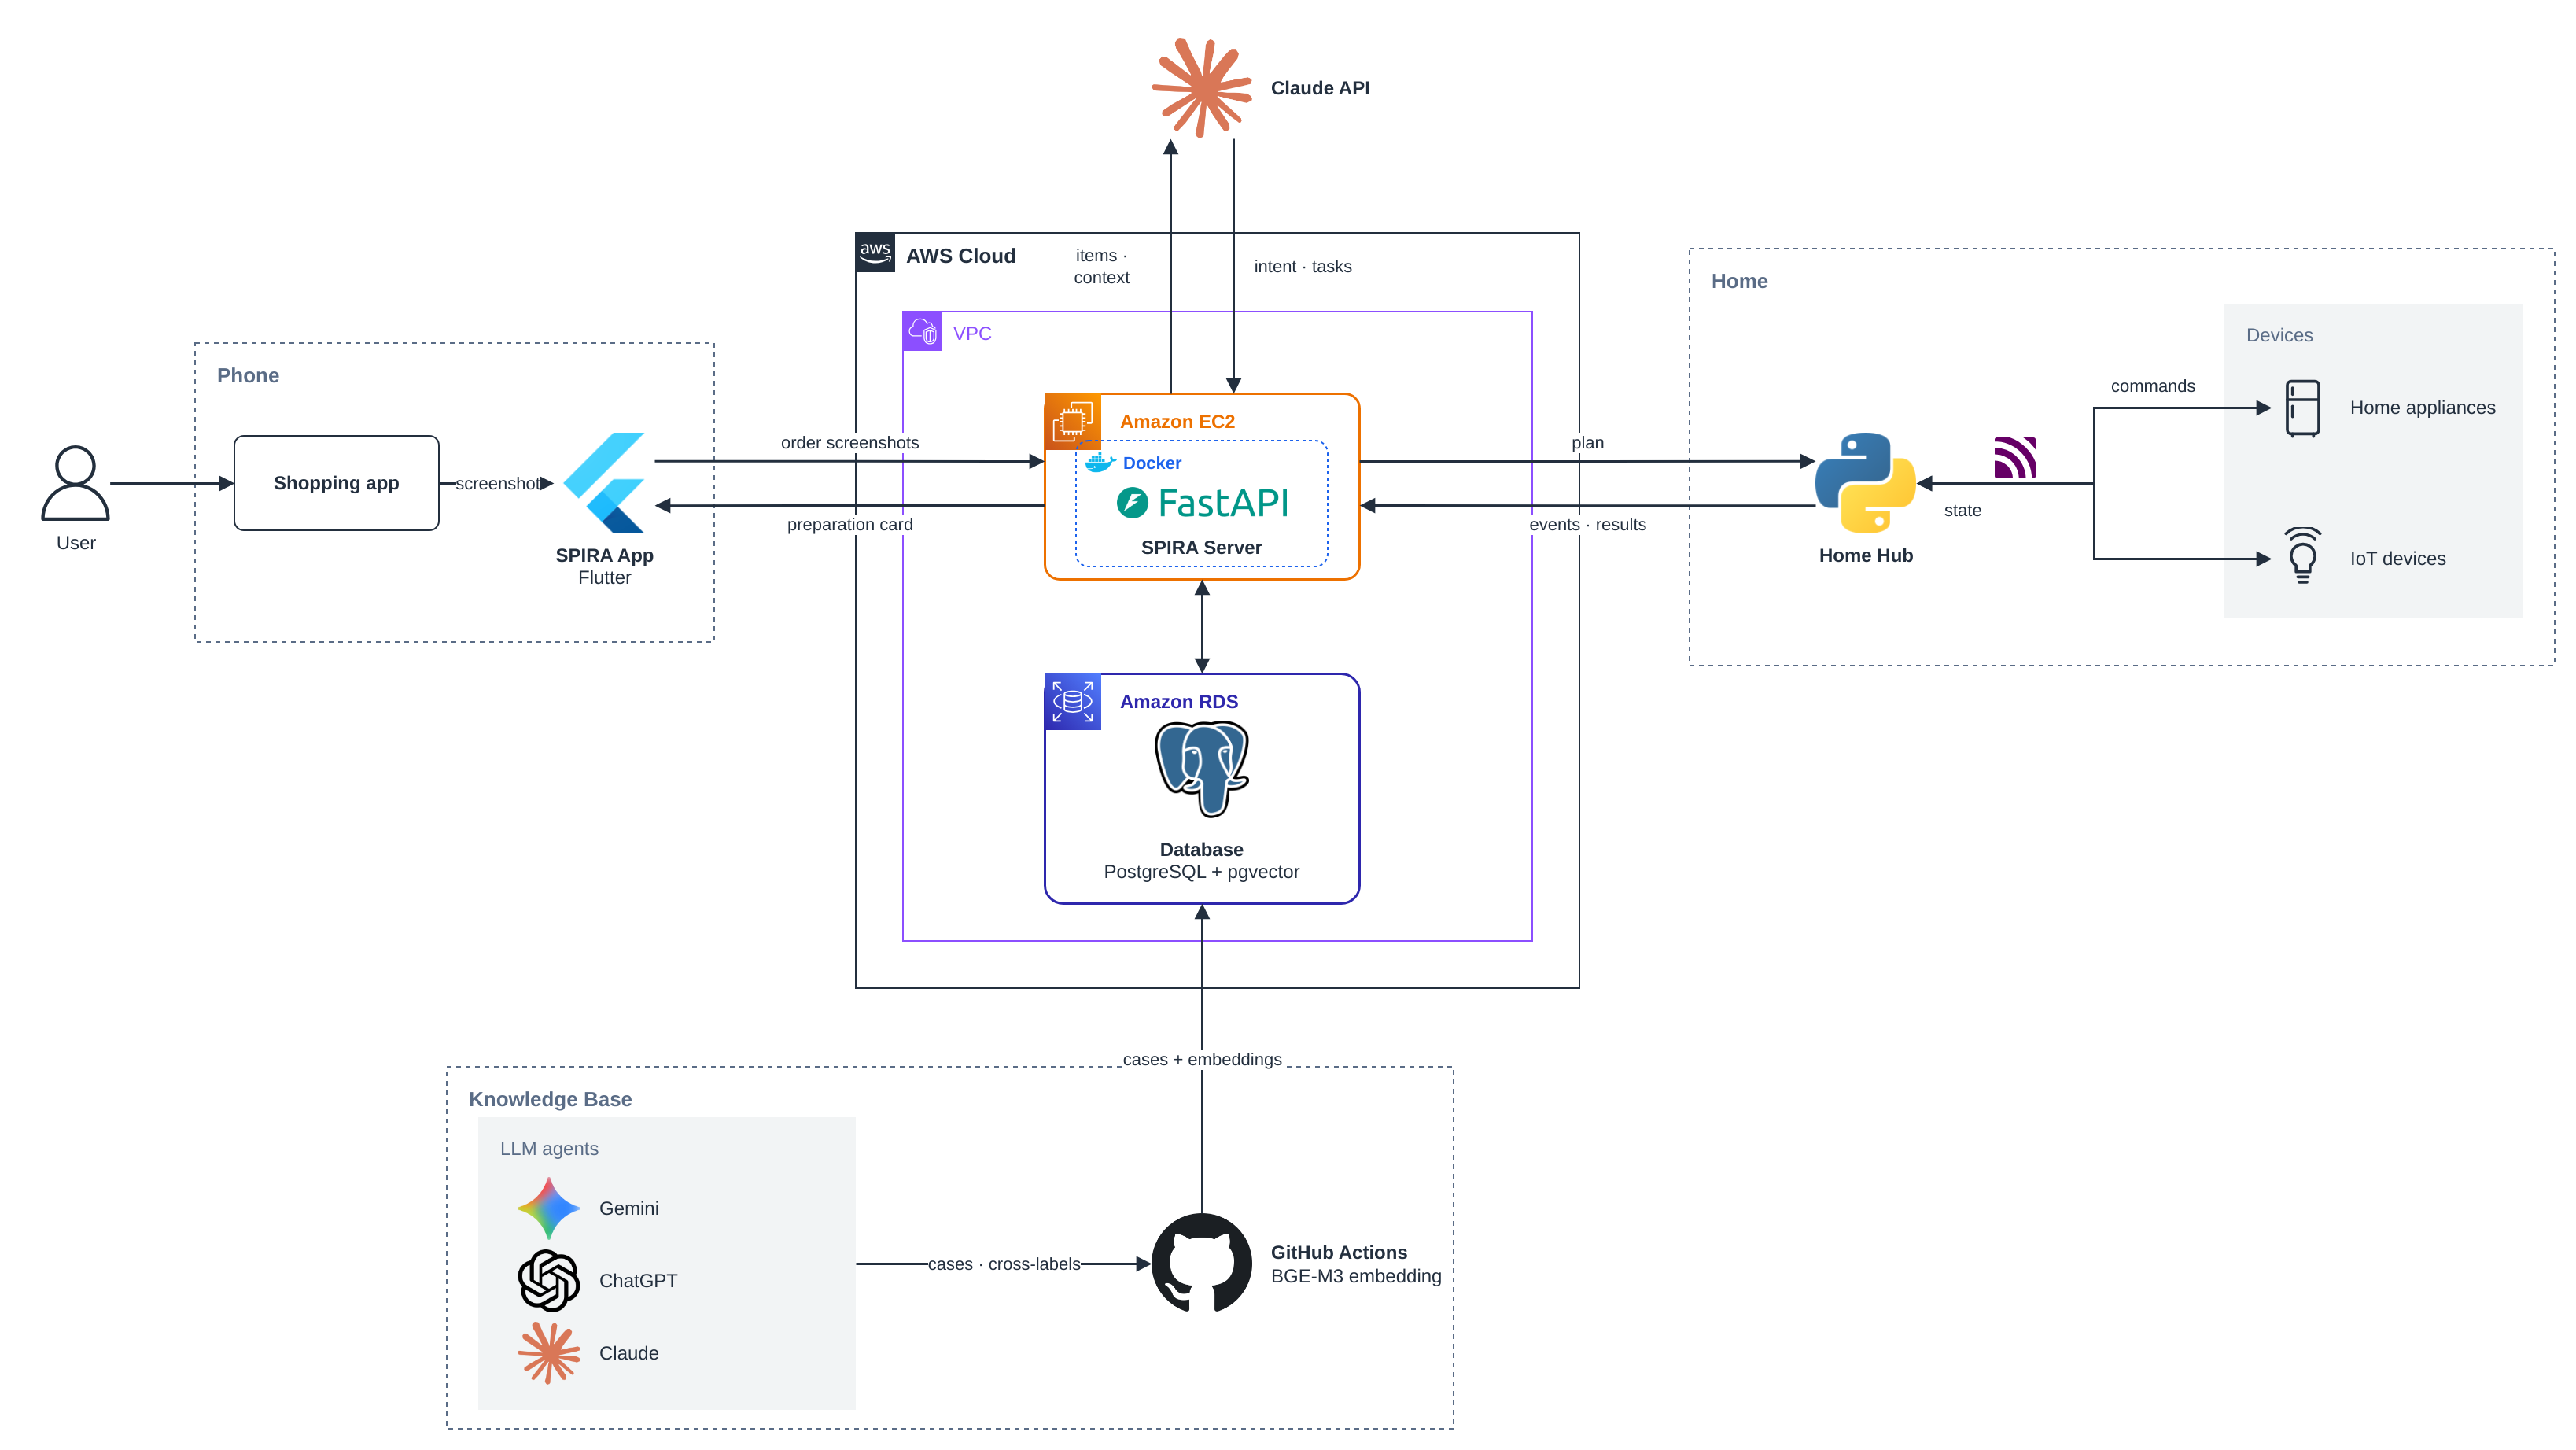
\includegraphics[width=\textwidth]{fig_architecture.png}
\caption{Overall architecture of SPIRA. Arrows show the direction of data. The AWS boundary (VPC, EC2, RDS) marks the planned deployment.}
\label{fig:arch}
\end{figure*}

\subsection{Directory Organization}
Table~\ref{tab:dirs} lists the source layout of the \texttt{CSE-SPIRA/SPIRA} repository and the separate knowledge-base repository.

\begin{table*}[!t]
\caption{Directory Organization}
\centering
\footnotesize
\setlength{\tabcolsep}{3pt}
\renewcommand{\arraystretch}{1.08}
\begin{tabularx}{\textwidth}{@{}L{0.20\textwidth}L{0.34\textwidth}L{0.13\textwidth}X@{}}
\toprule
\textbf{Directory} & \textbf{Main files} & \textbf{Module} & \textbf{Notes} \\
\midrule
\texttt{server/\allowbreak spira\_server/\allowbreak pipeline/} & \texttt{s1\_extract.py}, \texttt{s2\_context.py}, \texttt{s2\_calendar.py}, \texttt{s3\_intent.py}, \texttt{s4\_time.py}, \texttt{s4\_tasks.py}, \texttt{s5\_plan.py}, \texttt{s5\_cards.py}, \texttt{s5\_reactions.py}, \texttt{s6\_hub.py}, \texttt{s7\_observe.py}, \texttt{runner.py} & Server S1--S7 & One file per stage \\
\texttt{server/\allowbreak spira\_server/} & \texttt{api/}, \texttt{llm/}, \texttt{kb/}, \texttt{db/}, \texttt{scheduler.py}, \texttt{demo\_clock.py}, \texttt{prompts/*.txt} & Server API, model and KB access & Korean prompt originals \\
\texttt{server/config/} & \texttt{numbers.yaml}, \texttt{label\_table.yaml}, \texttt{item\_tasks.yaml}, \texttt{command\_policy.yaml}, \texttt{sensitive\_words.yaml}, \texttt{card\_templates.yaml}, \texttt{holiday\_calendar.yaml} & Server rules & Tables and numbers, not code \\
\texttt{server/\allowbreak migrations/} & Alembic versions & Server DB & PostgreSQL 16 + pgvector \\
\texttt{hub/\allowbreak spira\_hub/} & \texttt{plans.py}, \texttt{runtime.py}, \texttt{device.py}, \texttt{observations.py}, \texttt{store.py}, \texttt{dashboard.py}, \texttt{story\_clock.py} & Home Hub & SQLite store, MQTT device client \\
\texttt{app/lib/} & \texttt{main.dart}, \texttt{app\_controller.dart}, \texttt{api/app\_api.dart}, \texttt{features/} (setup, preparations, calendar, our home, memory), \texttt{platform/} (Android share, Google Calendar) & App & Flutter; share receiver in Kotlin under \texttt{app/android} \\
\texttt{simulator/\allowbreak spira\_simulator/} & \texttt{world.py}, \texttt{mqtt.py}, \texttt{api.py}, \texttt{surfaces.py}, \texttt{profiles/ep\_9031.json}, \texttt{profiles/ep\_9120.json}, \texttt{ui/} & Test home & Device truth, operator, viewer, judge \\
\texttt{contracts/} & \texttt{openapi/app.yaml}, \texttt{openapi/hub.yaml}, \texttt{schemas/*.json}, \texttt{kb/intents.json}, \texttt{fixtures/}, \texttt{generated/} & Shared contract & Generated Python and Dart models \\
\texttt{demo-shell/} & \texttt{demo.py}, \texttt{ui/}, \texttt{design/} (tokens, vocabulary) & Demonstration & Phone and Server judgment side by side \\
\texttt{docs/} & \texttt{architecture.md}, \texttt{paper.tex}, \texttt{paper.pdf} & Documentation & This paper \\
\texttt{SPIRA\_KB} (separate) & \texttt{config/pipeline.yaml}, \texttt{data/*/batches/}, embedding package \texttt{spira-kb} & Knowledge base & GitHub Actions; \texttt{kb-v1} tag \\
\bottomrule
\end{tabularx}
\label{tab:dirs}
\end{table*}

\subsection{SPIRA Server}
\textbf{Purpose.} The Server turns screenshots into a validated, versioned plan and turns what happened into household memory. It does not execute device commands, wait for triggers, restore devices, or create knowledge-base cases.

\textbf{Implementation.} All stages S1--S7 and the App and Hub routes of S6 are implemented in Python with FastAPI, together with a dry-run tool. S6 serves plans, Hub events, and execution results with card-line states, package release, task ends, and restores; S7 opens observation windows, records verdicts and per-line feedback, and writes household memory rows that the App can list and delete. For the demonstration, a story clock on the Server (\texttt{DEMO\_MODE}) gives the Server, Hub, and test home one shared time, and read-only routes expose each episode's stage trace. Each stage commits its result so an episode can resume after a restart, and a household lock orders concurrent inputs. The model client wraps one interface with providers and a mock; S1, calendar tagging, and S3 enforce JSON outputs, while S4 states its format in the prompt because its schema grows with the device list.

\textbf{Dry runs.} Two dry runs with real screenshots and \texttt{kb-v1} (2,080 cases at the time) produced eleven revisions (R40--R50). For example, a 0.6 similarity floor admitted all 200 neighbours of the birthday order, including cases sharing no item, so the floor was raised to 0.70; and reading the same cart photo twice produced ``birthday balloon'' once and ``balloon set'' once, which moved neighbours above the floor from 31 to 2, so S1 now keeps occasion words in item types. Later revisions (R51--R56) limit fridge notices to little-known care and to handling that the intent changes, and align S6 and S7 with the Hub's event format.

\subsection{Synthetic Purchase-Intent Knowledge Base}
\textbf{Purpose.} The knowledge base provides retrievable purchase-intent cases before real records exist.

\textbf{Process.} Lists are fixed first: 30 intents, 30 calendar tags, and 20 household types. Agents built on Gemini, Codex, and Claude generate order bundles; two models from different companies label each case without seeing each other's label; a GitHub Actions job (\texttt{spira tick}) assembles batches, compares labels, applies a quality gate, removes near duplicates above 0.97 similarity, embeds item lists with BGE-M3, and loads cases.

\textbf{Status.} The tag \texttt{kb-v1} contains the first-cycle batches A1 and B1; five of six batches recorded 5,166 loaded cases, and one batch records zero loaded rows, which is under review. All six first-cycle batches missed the automatic gate, mostly by small margins: on the B-type re-read metric, three batches scored 84.0--84.8\% against a starting threshold of 85\%, and every batch had three to five underproduced intents. The knowledge-base owner passed each batch with a written reason, as the design treats the first thresholds as starting values. Human review covered 30 cases per batch, with 0 to 3 of 30 labels judged wrong. The most frequent label disagreements were between an intent and \texttt{none} (e.g., home party versus none in 35 cases), which shows that deciding whether an order has an intent is harder than choosing among intents.

\subsection{Home Hub}
\textbf{Purpose.} The Hub turns plans into effects at the right home and time, observes what actually happened, and preserves person-made changes. It does not infer intent or choose targets or values.

\textbf{Implementation.} The Hub is a Python service with a SQLite store and an MQTT device client. It pulls and acknowledges plan versions, evaluates triggers, dispatches delegated commands, reads back state, tracks ownership per property, and restores owned properties at the end. It also exposes a dashboard of plans, executions, and evidence. Against a contract fixture Server, the App, Hub, and test home pass automated tests for three example days: a birthday, ordinary grocery shopping, and a visit to parents. On 2026-11-27 the Hub and test home were connected to the actual Server; the Hub installation and the test-home profile are generated from the Server's demonstration home.

\subsection{App}
\textbf{Purpose.} The App shares orders, shows preparation cards and their rationale, and provides the three interventions.

\textbf{Implementation.} The App is written in Flutter for Android. It receives shared images through a Kotlin share intent, reads Google Calendar events and sends them to the Server, polls cards every 30 seconds, shows card lines with their contract states, and accepts the card reactions. It also includes first-run onboarding (room and name confirmation of discovered devices and delegation defaults), a month calendar, an episode list, and household memory, and it runs against the actual Server in the demonstration phone.

\subsection{Test Home (Simulator) and Contracts}
\textbf{Test home.} The simulator holds the truth of each virtual device, accepts commands over MQTT, emits events such as package bring-in, guest arrival, and event end, and judges whether the Hub's reports match what happened. Household profiles reproduce the demonstration homes, and a web viewer shows the house.

\textbf{Contracts.} The \texttt{contracts/} folder fixes every value exchanged between parts: OpenAPI files for the App and Hub routes, JSON schemas for plans, cards, rationale, events, and memory rows, enums in English codes, the knowledge-base lists, and fixtures for the example episodes. Python and Dart models are generated from it, so a change is made once and checked in every part.

\section{Use Cases}
The use cases follow the contract fixtures in \texttt{contracts/fixtures/} (\texttt{ep\_9031}, \texttt{ep\_9120}), which the App, Hub, and test home already pass against the fixture Server. Screenshots will be added from the demonstration build.

\subsection{Use Case 1: Birthday Order (S1--S5, Hub)}
Satisfies order sharing, extraction, retrieval, intent judgment, time by code, task generation, plan validation, and execution.
\begin{enumerate}
\item On Thursday at 21:00 the user shares two cart screenshots to SPIRA through the Android share sheet.
\item Ten quiet minutes later the Server reads nine items (strawberries, cupcake mix, whipping cream, detergent, lotion, balloons, cake topper, party hats, icing pens), judges a child's birthday party, takes the time (Saturday 14:00--17:00) from the calendar, and publishes plan version 1 with one card of four lines: cleaning, child-safety mode, mood screen and light, and oven standby. Detergent and lotion stay outside the bundle.
\item The Hub pulls version 1 within 15 seconds and acknowledges it.
\item On Friday at 18:05 the test home reports the package brought in; the fridge screen shows the strawberry and whipping-cream notices.
\item On Saturday at 13:30 the cooktop child lock and the kettle plug-off run as protective tasks. At 13:52 the first guest arrives, and the display and light change. At 14:00 the oven is set to 170\,\textdegree{}C for 20 minutes in standby; at 14:20 a person starts it.
\end{enumerate}

\subsection{Use Case 2: Switching Off a Line and a Person's Change (S5, Hub, S7)}
Satisfies line control, plan versioning, ownership, restoration, and household memory.
\begin{enumerate}
\item On Friday morning the user switches off the cleaning line (``I'll clean myself''). The Server publishes version 2 with the cleaning task cancelled before it started.
\item During the party a person changes the light to 2700\,K.
\item At 17:50 the test home reports the event end. The Hub restores the display, keeps the light because a person changed it, and releases the child lock and kettle because the end was observed.
\item S7 closes the window with verdict \texttt{match} (the person started the oven left in standby) and feedback: cleaning \texttt{off}, safety \texttt{kept}, mood \texttt{changed}, oven \texttt{kept}. The next birthday order of this household leaves out cleaning for 180 days.
\end{enumerate}

\subsection{Use Case 3: Ordinary Grocery Order (S1--S4)}
Satisfies no-intent handling and per-item tasks.
\begin{enumerate}
\item The user shares an ordinary grocery cart (\texttt{ep\_9120}).
\item S3 returns no intent, so no preparation card is shown.
\item Per-item tasks still apply at package bring-in, for items that need care.
\end{enumerate}

\subsection{Use Case 4: Stop, Rationale, and Memory (App, S6)}
Satisfies the stop control, explanation, and memory deletion.
\begin{enumerate}
\item The user presses Stop on a card. Unstarted lines are cancelled, effects SPIRA still owns are restored, and person changes are kept; the App shows the request as pending until the next card state confirms it.
\item The user opens a card's rationale and sees the items, the intent, knowledge-base counts by intent, and each task with its device and room.
\item In settings the user lists this home's memory rows and deletes one; later preparation no longer uses it.
\end{enumerate}

\balance
\begin{thebibliography}{99}
\scriptsize
\bibitem{ref1}P. Sarantopoulos, A. Theotokis, K. Pramatari, and G. Doukidis, ``Shopping missions: An analytical method for the identification of shopper need states,'' \emph{Journal of Business Research}, vol. 69, no. 3, pp. 1043--1052, 2016, doi: \href{https://doi.org/10.1016/j.jbusres.2015.08.017}{10.1016/j.jbusres.2015.08.017}.
\bibitem{ref2}Z. Sun, J. Yang, K. Feng, H. Fang, X. Qu, and Y. S. Ong, ``Revisiting bundle recommendation: Datasets, tasks, challenges and opportunities for intent-aware product bundling,'' in \emph{Proceedings of the 45th International ACM SIGIR Conference on Research and Development in Information Retrieval}, 2022, pp. 2900--2911, doi: \href{https://doi.org/10.1145/3477495.3531904}{10.1145/3477495.3531904}.
\bibitem{ref3}Z. Sun, K. Feng, J. Yang, X. Qu, H. Fang, Y.-S. Ong, and W. Liu, ``Adaptive in-context learning with large language models for bundle generation,'' in \emph{Proceedings of the 47th International ACM SIGIR Conference on Research and Development in Information Retrieval}, 2024, pp. 966--976, doi: \href{https://doi.org/10.1145/3626772.3657808}{10.1145/3626772.3657808}.
\bibitem{ref4}C. Yu, X. Liu, J. Maia, T. Cao, L. Li, Y. Gao, Y. Song, R. Goutam, H. Zhang, B. Yin, and Z. Li, ``COSMO: A large-scale e-commerce common sense knowledge generation and serving system at Amazon,'' in \emph{Companion Proceedings of the 2024 International Conference on Management of Data}, 2024, doi: \href{https://doi.org/10.1145/3626246.3653398}{10.1145/3626246.3653398}.
\bibitem{ref5}S. Zeng, J. Zhang, P. He, J. Ren, T. Zheng, H. Lu, H. Xu, H. Liu, Y. Xing, and J. Tang, ``Mitigating the privacy issues in retrieval-augmented generation via pure synthetic data,'' in \emph{Proceedings of the 2025 Conference on Empirical Methods in Natural Language Processing}, 2025, pp. 24527--24558, doi: \href{https://doi.org/10.18653/v1/2025.emnlp-main.1247}{10.18653/v1/2025.emnlp-main.1247}.
\bibitem{ref6}A. Salemi, S. Mysore, M. Bendersky, and H. Zamani, ``LaMP: When large language models meet personalization,'' in \emph{Proceedings of the 62nd Annual Meeting of the Association for Computational Linguistics, Volume 1: Long Papers}, 2024, pp. 7370--7392, doi: \href{https://doi.org/10.18653/v1/2024.acl-long.399}{10.18653/v1/2024.acl-long.399}.
\bibitem{ref7}E. King, H. Yu, S. Lee, and C. Julien, ``Sasha: Creative goal-oriented reasoning in smart homes with large language models,'' \emph{Proceedings of the ACM on Interactive, Mobile, Wearable and Ubiquitous Technologies}, vol. 8, no. 1, article 12, pp. 1--38, 2024, doi: \href{https://doi.org/10.1145/3643505}{10.1145/3643505}.
\bibitem{ref8}S. Li, Y. Guo, J. Yao, Z. Liu, and H. Wang, ``HomeBench: Evaluating LLMs in smart homes with valid and invalid instructions across single and multiple devices,'' in \emph{Proceedings of the 63rd Annual Meeting of the Association for Computational Linguistics, Volume 1: Long Papers}, 2025, pp. 12230--12250, doi: \href{https://doi.org/10.18653/v1/2025.acl-long.597}{10.18653/v1/2025.acl-long.597}.
\bibitem{ref9}Python Software Foundation, ``Status of Python versions.'' [Online]. Available: https://devguide.python.org/versions/.
\bibitem{ref10}FastAPI, ``fastapi.'' \emph{Python Package Index}. [Online]. Available: https://pypi.org/project/fastapi/.
\bibitem{ref11}M. Trylesinski and contributors, ``uvicorn.'' \emph{Python Package Index}. [Online]. Available: https://pypi.org/project/uvicorn/.
\bibitem{ref12}PostgreSQL Global Development Group, ``PostgreSQL versioning policy.'' [Online]. Available: https://www.postgresql.org/support/versioning/.
\bibitem{ref13}pgvector contributors, ``pgvector changelog.'' [Online]. Available: https://github.com/pgvector/pgvector/blob/master/CHANGELOG.md.
\bibitem{ref14}Flutter, ``Install Flutter manually.'' [Online]. Available: https://docs.flutter.dev/install/manual.
\bibitem{ref15}J. Chen, S. Xiao, P. Zhang, K. Luo, D. Lian, and Z. Liu, ``BGE M3-embedding: Multi-lingual, multi-functionality, multi-granularity text embeddings through self-knowledge distillation,'' arXiv:2402.03216, 2024.
\bibitem{ref16}A. Panickssery, S. R. Bowman, and S. Feng, ``LLM evaluators recognize and favor their own generations,'' in \emph{Advances in Neural Information Processing Systems 37}, 2024.
\end{thebibliography}
\end{document}
